% Options for packages loaded elsewhere
\PassOptionsToPackage{unicode}{hyperref}
\PassOptionsToPackage{hyphens}{url}
\PassOptionsToPackage{dvipsnames,svgnames,x11names}{xcolor}
%
\documentclass[
]{article}
\title{Practical Work}
\usepackage{etoolbox}
\makeatletter
\providecommand{\subtitle}[1]{% add subtitle to \maketitle
  \apptocmd{\@title}{\par {\large #1 \par}}{}{}
}
\makeatother
\subtitle{Lifetime Data Analysis}
\author{Rodrigo Arriaza, Alexander J Ohrt}
\date{07 January, 2022}

\usepackage{amsmath,amssymb}
\usepackage{lmodern}
\usepackage{iftex}
\ifPDFTeX
  \usepackage[T1]{fontenc}
  \usepackage[utf8]{inputenc}
  \usepackage{textcomp} % provide euro and other symbols
\else % if luatex or xetex
  \usepackage{unicode-math}
  \defaultfontfeatures{Scale=MatchLowercase}
  \defaultfontfeatures[\rmfamily]{Ligatures=TeX,Scale=1}
\fi
% Use upquote if available, for straight quotes in verbatim environments
\IfFileExists{upquote.sty}{\usepackage{upquote}}{}
\IfFileExists{microtype.sty}{% use microtype if available
  \usepackage[]{microtype}
  \UseMicrotypeSet[protrusion]{basicmath} % disable protrusion for tt fonts
}{}
\makeatletter
\@ifundefined{KOMAClassName}{% if non-KOMA class
  \IfFileExists{parskip.sty}{%
    \usepackage{parskip}
  }{% else
    \setlength{\parindent}{0pt}
    \setlength{\parskip}{6pt plus 2pt minus 1pt}}
}{% if KOMA class
  \KOMAoptions{parskip=half}}
\makeatother
\usepackage{xcolor}
\IfFileExists{xurl.sty}{\usepackage{xurl}}{} % add URL line breaks if available
\IfFileExists{bookmark.sty}{\usepackage{bookmark}}{\usepackage{hyperref}}
\hypersetup{
  pdftitle={Practical Work},
  pdfauthor={Rodrigo Arriaza, Alexander J Ohrt},
  colorlinks=true,
  linkcolor={Maroon},
  filecolor={Maroon},
  citecolor={Blue},
  urlcolor={blue},
  pdfcreator={LaTeX via pandoc}}
\urlstyle{same} % disable monospaced font for URLs
\usepackage[margin=1in]{geometry}
\usepackage{longtable,booktabs,array}
\usepackage{calc} % for calculating minipage widths
% Correct order of tables after \paragraph or \subparagraph
\usepackage{etoolbox}
\makeatletter
\patchcmd\longtable{\par}{\if@noskipsec\mbox{}\fi\par}{}{}
\makeatother
% Allow footnotes in longtable head/foot
\IfFileExists{footnotehyper.sty}{\usepackage{footnotehyper}}{\usepackage{footnote}}
\makesavenoteenv{longtable}
\usepackage{graphicx}
\makeatletter
\def\maxwidth{\ifdim\Gin@nat@width>\linewidth\linewidth\else\Gin@nat@width\fi}
\def\maxheight{\ifdim\Gin@nat@height>\textheight\textheight\else\Gin@nat@height\fi}
\makeatother
% Scale images if necessary, so that they will not overflow the page
% margins by default, and it is still possible to overwrite the defaults
% using explicit options in \includegraphics[width, height, ...]{}
\setkeys{Gin}{width=\maxwidth,height=\maxheight,keepaspectratio}
% Set default figure placement to htbp
\makeatletter
\def\fps@figure{htbp}
\makeatother
\setlength{\emergencystretch}{3em} % prevent overfull lines
\providecommand{\tightlist}{%
  \setlength{\itemsep}{0pt}\setlength{\parskip}{0pt}}
\setcounter{secnumdepth}{5}
\usepackage{float}
\usepackage{booktabs}
\usepackage{longtable}
\usepackage{array}
\usepackage{multirow}
\usepackage{wrapfig}
\usepackage{float}
\usepackage{colortbl}
\usepackage{pdflscape}
\usepackage{tabu}
\usepackage{threeparttable}
\usepackage{threeparttablex}
\usepackage[normalem]{ulem}
\usepackage{makecell}
\usepackage{xcolor}
\ifLuaTeX
  \usepackage{selnolig}  % disable illegal ligatures
\fi

\begin{document}
\maketitle

\hypertarget{introduction}{%
\section{Introduction}\label{introduction}}

We are given a data set on sexually transmitted diseases (STDs). This is data from a study about gonorrhea and chlamydia in 877 women. The objective with this practical work is to study possible risk factors for a reinfection with gonorrhea or chlamydia in women who have suffered one or both infections previously. The variables of interest are sociodemographic variables or those related to sexual practice. We have a lot of variables at our disposal, but have chosen to use the following, some for statistical reasons and some for medical reasons:

\begin{itemize}
\tightlist
\item
  Age: The age of the woman.
\item
  NumPartners: The number of partners during the last 30 days.
\item
  CondomUse: Use of condoms (1: always, 2: once in a while, 3: never)
\item
  YearsSchool: Years of schooling.
\item
  InitInfect: Initial infection (1: Gonorrhea, 2: Chlamydia, 3: both)
\item
  InvVagAtExam: Involvement vagina at exam (1: yes; 0: no).
\item
  DischargeExam: Discharge at exam (1: yes; 0: no)
\end{itemize}

The first three were chosen based on results from a \href{https://www.ncbi.nlm.nih.gov/pmc/articles/PMC1744639/}{study} on gonorrhea reinfection in heterosexual STD clinic attendees. The study concluded that increased reinfection risk (of gonorrhea) was associated with younger age and a greater number of recent sex partners, among other risk factors. Moreover, the authors concluded that any type of condom use was a risk factor for reinfection with gonorrhea in women.

Another \href{https://policylab.chop.edu/sites/default/files/pdf/publications/Preventing_Chlamydia_Gonorrhea_Reinfection_through_Increased_Use_of_EPT.pdf}{publication} reports that, on average, 14\% of women with clamydia and 12\% of women with gonorrhea get reinfected, with younger women at higher risk. Moreover, they state that many adolescents treated for infection of one of the two STDs are reinfected within three to six months, usually because of resumed sexual contact with an untreated partner. Thus, the marital status might be interesting to analyse. However, this is not added, because, the ages in the data set are low, which most likely means that the amount in each level of \texttt{MaritalStatus} is very skewed towards ``single''. This can be seen in the descriptive analysis below.

\href{https://www.ncbi.nlm.nih.gov/pmc/articles/PMC2094865/}{This meta-analysis} reports that the relationship between race, socioeconomic status (SES) and chlamydial infection is not clear. It concludes that SES was not associated with chlamydia infection, when they tested for several variables, where level of parent's education was one of them. Either way, we think it might be interesting to see if the years of schooling of the women (\texttt{YearsSchool}) have any impact on reinfection. Moreover, as will be shown below, the covariate \texttt{YearsSchool} is statistically significant according to the given model.

We also chose to use the initial infection (\texttt{InitInfect}) as an explanatory variable, because several of the studies above are only done on one of the two diseases, not on both at the same time. Because of this we wanted to investigate if the initial infection type is a risk factor and, if this is the case, if the risk differs based on which infection was suffered initially.

\hypertarget{statistical-variable-selection}{%
\subsection{Statistical Variable Selection}\label{statistical-variable-selection}}

As noted, in addition to medical criteria for selecting variables, we have used a negative binomial model to discover which variables are statistically significant to the event of reinfection. The negative binomial model can be fitted when the occurence of events is a count for each patient, as described in \href{https://pubmed.ncbi.nlm.nih.gov/22083507/}{this article}. Fitting a negative binomial generalized linear model, with the canonical link, with all the variables in the data set and converting the time until reinfection into an offset, yields the parameter estimates and \(p\)-values shown in table \ref{tab:variable-select}. Note that the time until reinfection is converted into an offset because we are comparing counts for different follow-up times (a person that has been in the study longer would have higher chances of getting reinfected).

\begin{table}

\caption{\label{tab:variable-select}Statistical significance of the variables using a negative binomial model}
\centering
\begin{tabular}[t]{l|r|r}
\hline
  & Estimate & Pr(>|z|)\\
\hline
(Intercept) & -4.4766626 & 0.0000000\\
\hline
EthnicityW & -0.0786114 & 0.6179527\\
\hline
MaritalStatusM & 0.1142920 & 0.8071114\\
\hline
MaritalStatusS & 0.5011754 & 0.1177317\\
\hline
Age & 0.0188481 & 0.2273932\\
\hline
\cellcolor{blue}{\textcolor{white}{YearsSchool}} & \cellcolor{blue}{\textcolor{white}{-0.1689015}} & \cellcolor{blue}{\textcolor{white}{0.0001358}}\\
\hline
InitInfect2 & -0.3302518 & 0.0578210\\
\hline
InitInfect3 & -0.3318821 & 0.0587288\\
\hline
NumPartners & 0.1164568 & 0.0516276\\
\hline
OralSex12m1 & -0.3703474 & 0.1208812\\
\hline
OralSex30d1 & -0.3246975 & 0.2193066\\
\hline
RectalSex12m1 & 0.0669703 & 0.8908790\\
\hline
RectalSex30d1 & -0.1627456 & 0.7920361\\
\hline
AbPain1 & 0.2969178 & 0.0937042\\
\hline
SignDischarge1 & 0.1330009 & 0.3087416\\
\hline
SignDysuria1 & 0.1954606 & 0.2808455\\
\hline
CondomUse2 & -0.1553543 & 0.5686201\\
\hline
CondomUse3 & -0.4582270 & 0.1041693\\
\hline
SignItch1 & -0.2209724 & 0.2068424\\
\hline
SignLesion1 & -0.2541307 & 0.5021878\\
\hline
SignRash1 & -0.0638066 & 0.8895122\\
\hline
SignLymph1 & 0.2368538 & 0.6892069\\
\hline
\cellcolor{blue}{\textcolor{white}{InvVagAtExam1}} & \cellcolor{blue}{\textcolor{white}{0.5726933}} & \cellcolor{blue}{\textcolor{white}{0.0042620}}\\
\hline
\cellcolor{blue}{\textcolor{white}{DischargeExam1}} & \cellcolor{blue}{\textcolor{white}{-0.5805191}} & \cellcolor{blue}{\textcolor{white}{0.0310111}}\\
\hline
AbnormNodeExam1 & 0.0801562 & 0.8764938\\
\hline
\end{tabular}
\end{table}

This model explains why the vaginal involvement at exam (\texttt{InvVagAtExam}) and the discharge at exam (\texttt{DischargeExam}) are selected as variables in our analysis, since they are shown as statistically significant in Table \ref{tab:variable-select}.

\hypertarget{descriptive-analysis}{%
\section{Descriptive Analysis}\label{descriptive-analysis}}

In total, the data set contains 24 variables, but, as noted, we have selected only 7 of them in our analysis. Recall that the data set has 877 women. The percentage of right-censored data in the data set is 60.4, which is a relatively large part of the data set. The women where followed for 1529 days, then the study was stopped. For women that were initially infected with only gonorrhea, 8.32\% were reinfected, while for women that were initially infected with only chlamydia, 15.39\% were reinfected. Finally, for women that were initially infected with both diseases, 15.85\% were reinfected.

\begin{figure}
\centering
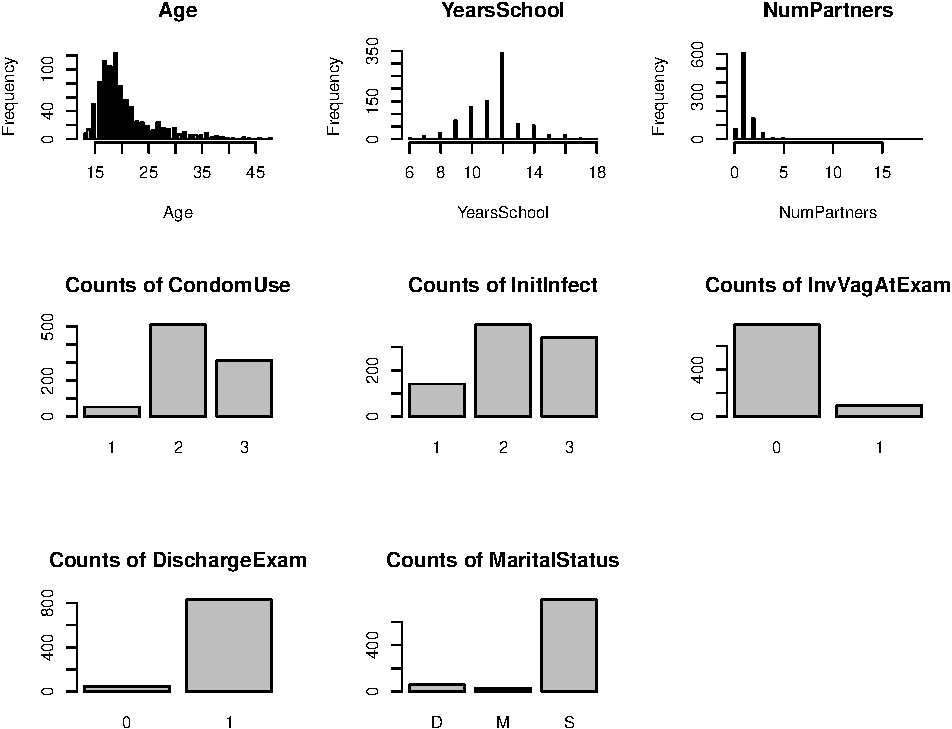
\includegraphics{practical_files/figure-latex/EDA-plots-1.pdf}
\caption{\label{fig:EDA-plots}Distributions of variables in the data set}
\end{figure}

The three continuous variables we have chosen to use in the analysis are \texttt{Age}, \texttt{YearsSchool} and \texttt{NumPartners}. The correlations between these variables are not significant except between \texttt{Age} and \texttt{YearsSchool} with the value of 0.43. This could be interesting to have in mind in the following.

\hypertarget{nonparametric-analysis}{%
\section{Nonparametric Analysis}\label{nonparametric-analysis}}

\hypertarget{survival-curve-estimation}{%
\subsection{Survival Curve Estimation}\label{survival-curve-estimation}}

The survival curve is estimated by means of Kaplan-Meier and plotted in figure \ref{fig:survivalf}. The curve shows the general survival in the data set.

\begin{figure}
\centering
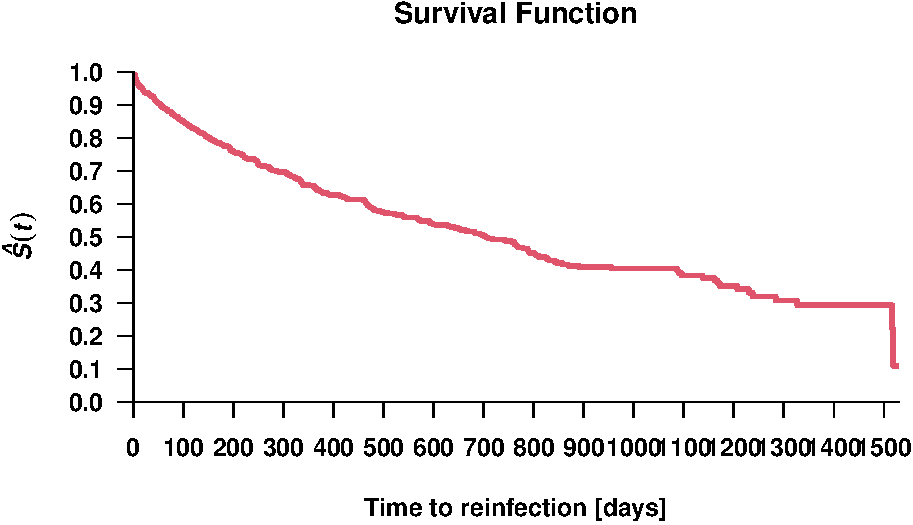
\includegraphics{practical_files/figure-latex/survivalf-1.pdf}
\caption{\label{fig:survivalf}Survival function of time until reinfection}
\end{figure}

The median survival time is estimated to be 705 days.

\hypertarget{comparison-of-survival-curves}{%
\subsection{Comparison of Survival Curves}\label{comparison-of-survival-curves}}

Survival functions for different levels of the nominal variables are compared by means of the nonparametric logrank test. Note that other types of tests also can be used (Fleming-Harrington family of tests), but we have only used the logrank test in this case. The general \(k\)-sample hypothesis that is tested is

\begin{equation*}
        H_0: S_1(t) = \ldots = S_k(t), \forall t \leq \tau \text{ vs. } H_1: \text{ some } S_i(t) \neq S_l(t), \text{ for some } t \leq \tau,
\end{equation*}

where \(\tau\) is the chosen limit of the time of examination and \(k\) varies depending on the levels of the explanatory variable we are testing. The \(p\)-values from each of the tests are given in table \ref{tab:pvalues}. For instance, choosing a significance level of \(\alpha = 0.05\), we would conclude that reinfection depends on the level of \texttt{CondomUse}, \texttt{InitInfect} and \texttt{InvVagAtExam}, but that there is not enough evidence to conclude that reinfection depends on the level of \texttt{DischargeExam}.

\begin{table}

\caption{\label{tab:pvalues}p-values from logrank tests}
\centering
\begin{tabular}[t]{l|c|c|c|c}
\hline
  & CondomUse & InitInfect & InvVagAtExam & DischargeExam\\
\hline
p-values & 0.0132506 & 0.0145266 & 0.0068009 & 0.0558044\\
\hline
\end{tabular}
\end{table}

\hypertarget{fit-of-a-parametric-survival-model}{%
\section{Fit of a parametric survival model}\label{fit-of-a-parametric-survival-model}}

After trying to fit Weibull, log-logistic and lognormal log-linear models, we concluded that the Weibull model is best suited to our data.

\begin{figure}

{\centering 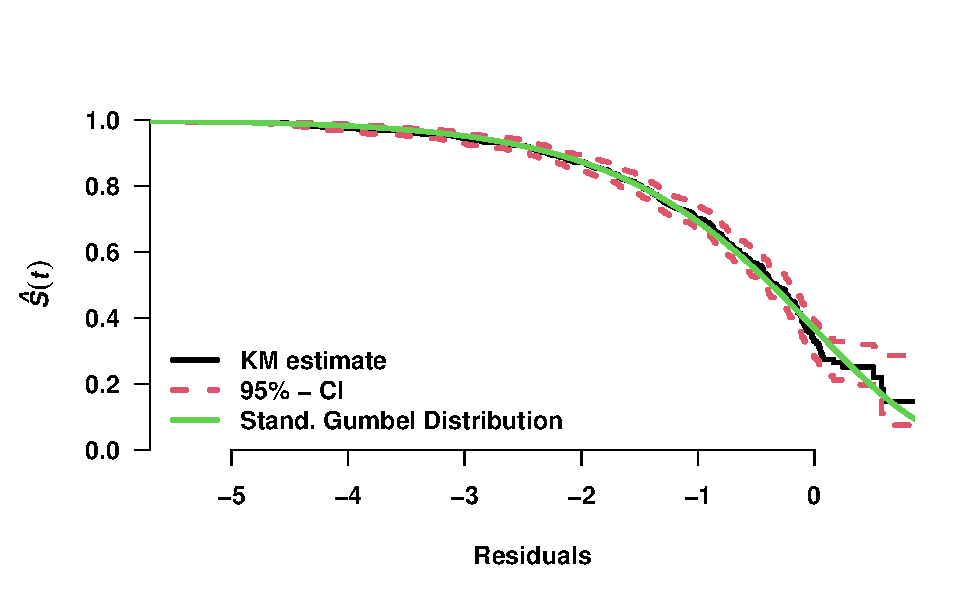
\includegraphics{practical_files/figure-latex/weibull-resids-1} 

}

\caption{Residuals of the Weibull Regression Model}\label{fig:weibull-resids}
\end{figure}

As seen in figure \ref{fig:weibull-resids}, the standard Gumbel distribution seems to fit relatively nicely to the Kaplan-Meier estimate of the residuals, i.e.~it seems like a reasonable choice for the error term \(W\), which indicates that the Weibull is a reasonable model.

\begin{figure}
\centering
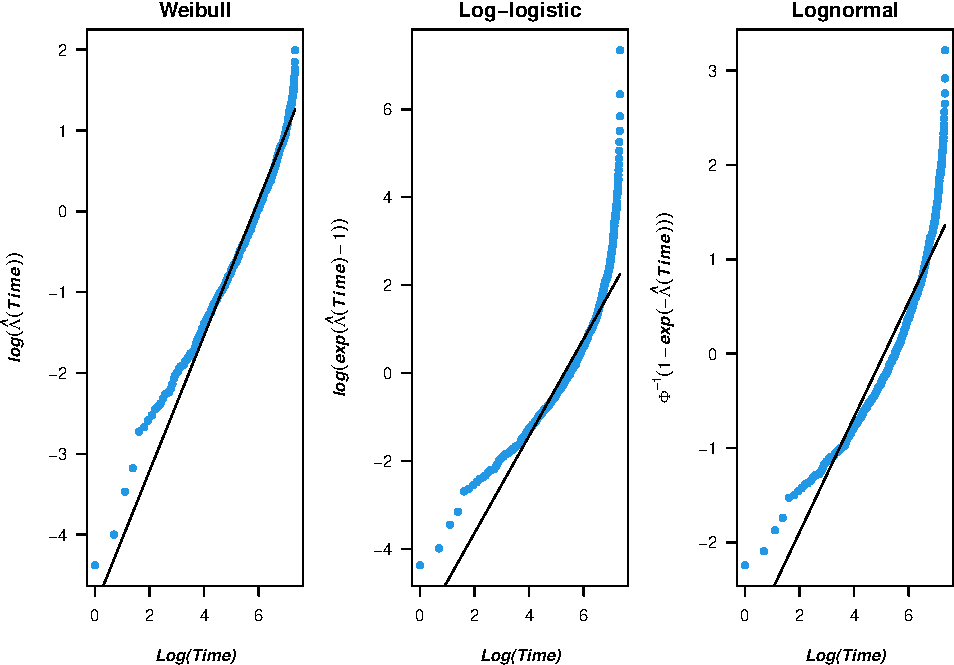
\includegraphics{practical_files/figure-latex/cumhaz-plot-1.pdf}
\caption{\label{fig:cumhaz-plot}Cumulative hazard plots comparison}
\end{figure}

The probability plots in figure \ref{fig:cumhaz-plot} also show that the Weibull is the better parametric model for the data, because the log-logistic and lognormal models clearly do not fit the line in the tails.

\hypertarget{interpretation}{%
\subsection{Interpretation}\label{interpretation}}

How do we interpret this model fit? First of all, the model we have fit follows the expression

\[
Y = \ln(T) = \mu + \mathbf{\gamma}^T\mathbf{Z} + \sigma W,  
\]

where \(W \sim EV(0,1)\),

\[
\mathbf{\gamma}^T = (\gamma_{Age}, \gamma_{NumPartn.}, \gamma_{Cond.}, \gamma_{YSchool}, \gamma_{InitInf.}, \gamma_{InvVagAtExam.}, \gamma_{DischargeAtExam}),
\]

are the estimated parameters and

\[
\mathbf{Z}^T = (Age, NumPartn., Cond., YSchool, InitInf., InvVagAtExam., DischargeAtExam), 
\]

is the vector of values. Thus, each of the quantities \(\exp(\gamma_i)\) can be interpreted as the unitary change in time until reinfection (when covariate \(i\) is continuous), or the change in time until reinfection when changing level (when the covariate \(i\) is nominal), when all the other explanatory variables are kept fixed. This means that a positive parameter estimate \(\hat{\gamma}_i\) gives \(\exp(\hat{\gamma}_i) > 0\), which means that the covariate is estimated to being protective by the model, since it increases \(\ln(T)\). The opposite holds for \(\hat{\gamma}_i < 0\). These interpretations will be done with the acceleration factor and relative hazard next.

In the Weibull model, the acceleration factor (AF) is calculated using the equation

\[
AF = \exp(-\hat{\gamma}_i),
\]
and the hazard ratio (HR) is calculated using the equation

\[
HR = \exp(-\hat{\gamma}_i/\hat{\sigma}).
\]
In this case, the model fit gives the scale \(\hat{\sigma} \approx\) 1.298. These values are calculated for each of the covariates and displayed in table \ref{tab:Weibull-table}.

\begin{table}

\caption{\label{tab:Weibull-table}Parameter estimates, p-values, AF and HR for the Weibull model}
\centering
\begin{tabular}[t]{l|r|r|r|r}
\hline
  & Parameter.Estimate & p & AF & HR\\
\hline
(Intercept) & 3.9516047 & 0.0000000 & 0.0192238 & 0.0475893\\
\hline
Age & 0.0101018 & 0.5291236 & 0.9899491 & 0.9922457\\
\hline
NumPartners & -0.0138832 & 0.8383511 & 1.0139800 & 1.0107560\\
\hline
CondomUse2 & 0.0788112 & 0.7924374 & 0.9242144 & 0.9410747\\
\hline
CondomUse3 & 0.4227912 & 0.1734952 & 0.6552154 & 0.7219443\\
\hline
YearsSchool & 0.1704370 & 0.0004676 & 0.8432962 & 0.8769191\\
\hline
InitInfect2 & 0.5109972 & 0.0073776 & 0.5998971 & 0.6745026\\
\hline
InitInfect3 & 0.3149121 & 0.1001146 & 0.7298530 & 0.7845268\\
\hline
InvVagAtExam1 & -0.5091714 & 0.0213272 & 1.6639119 & 1.4804896\\
\hline
DischargeExam1 & 0.4601294 & 0.1118362 & 0.6312020 & 0.7014676\\
\hline
\end{tabular}
\end{table}

Consider an example using the covariate \texttt{CondomUse} when explaining the interpretation of the covariates in terms of the AF. From the table it is apparent that the AF of \texttt{CondomUse3} versus \texttt{CondomUse1} is \(\approx\) 0.655. This means that the reinfection time for a person that never uses a condom is \(\approx\) 0.655 times the reinfection time for a person that always uses a condom. However as we have seen in table \ref{tab:variable-select}, the use of a condom was not statistically significant for this study, so it is uncertain to make conclusions such as this. More importantly, the fitted Weibull model gives large \(p\)-values for the levels of \texttt{CondomUse}, which leads to the same conclusion; that according to these statistical models, evidence of different risk of reinfection for the use of condoms does not exist. The interpretation in terms of the AF is similar when considering the other covariates, except for when considering the \texttt{Age} and \texttt{NumPartners}, which are not categorical. In these cases we talk about a similar change in the survival, i.e.~the reinfection time, for unitary changes in the covariates, when the rest of the profile is kept constant.

Similarly, an example can be used to explain the interpretation of the covariates in terms of the relative hazard. From the table it is apparent that the hazard of \texttt{CondomUse3} relative to \texttt{CondomUse1} is \(\approx\) 0.722. This means that the instantaneous risk of reinfection for a person that never uses a condom is \(\approx\) 0.722 times the instantaneous risk of a person that always uses a condom. Similar interpretations can be done with the other covariates.

\hypertarget{fit-of-a-semi-parametric-survival-model}{%
\section{Fit of a semi-parametric survival model}\label{fit-of-a-semi-parametric-survival-model}}

The fit of the proportional hazards model is shown in table \ref{tab:Cox-model}.

\begin{table}

\caption{\label{tab:Cox-model}Cox model fit}
\centering
\begin{tabular}[t]{l|r|r|r|r|r}
\hline
  & coef & exp(coef) & se(coef) & z & Pr(>|z|)\\
\hline
Age & -0.0078310 & 0.9921996 & 0.0123789 & -0.6326050 & 0.5269916\\
\hline
NumPartners & 0.0111954 & 1.0112583 & 0.0524833 & 0.2133127 & 0.8310831\\
\hline
CondomUse2 & -0.0551952 & 0.9463004 & 0.2312173 & -0.2387156 & 0.8113261\\
\hline
CondomUse3 & -0.3357060 & 0.7148332 & 0.2394857 & -1.4017788 & 0.1609813\\
\hline
YearsSchool & -0.1335637 & 0.8749717 & 0.0374028 & -3.5709522 & 0.0003557\\
\hline
InitInfect2 & -0.3868021 & 0.6792255 & 0.1464841 & -2.6405740 & 0.0082766\\
\hline
InitInfect3 & -0.2350049 & 0.7905670 & 0.1476823 & -1.5912871 & 0.1115450\\
\hline
InvVagAtExam1 & 0.4019162 & 1.4946861 & 0.1704810 & 2.3575432 & 0.0183963\\
\hline
DischargeExam1 & -0.3674385 & 0.6925059 & 0.2232460 & -1.6458903 & 0.0997863\\
\hline
\end{tabular}
\end{table}

\hypertarget{interpretation-1}{%
\subsection{Interpretation}\label{interpretation-1}}

How do we interpret this model fit? First of all, the model we have fit follows the expression

\[
\lambda(t|\mathbf{Z}) =  \exp(\mathbf{\beta}^T\mathbf{Z})\lambda_0(t),  
\]

where \(\beta\) are the parameters in the model and \(\mathbf{Z}\) is the profile of the woman. Additionally, \(\lambda_0(t)\) is the hazard at time \(t\) for a woman with profile \(\mathbf{Z} = 0\), i.e.~a woman that always uses a condom, that was initially infected with (only) gonorrhea, that did not experience vaginal involvement at exam and did not experience discharge at exam. The model assumes that the hazard ratio is proportionally equal to \(\exp(\mathbf{\beta}^T\mathbf{Z})\) at all times. Said in other words, it relates the instantaneous risk for a woman with profile \(\mathbf{Z}\) at time \(t\) with the instantaneous risk for a woman with the baseline profile at the same time \(t\). Each of the quantities \(\exp(\beta_i)\) can be interpreted as the unitary change in the proportion of the instanteneous risk (when covariate \(i\) is continuous), or the change in the proportion of the instanteneous risk when changing level (when the covariate \(i\) is nominal), when all the other explanatory variables are kept fixed. Remember that these proportions are calculated with \(\lambda_0(t)\) as the baseline. This means that a positive parameter estimate \(\hat{\beta}_i\) gives \(\exp(\hat{\beta}_i) > 0\), which means that the covariate is estimated to being a risk-factor by the model, since the proportion \(\frac{\lambda(t|\mathbf{Z} = z_i = 1)}{\lambda_0(t)} > 1\). The opposite holds for \(\hat{\beta}_i < 0\). Note that the notation \(\mathbf{Z} = z_i = 1\) used here refers to a vector \(\mathbf{Z}\) that has zero in all components except in component \(i\), where it has the value \(1\).

The model parameters \(\beta\) can be interpreted in terms of relative hazards. As is seen from the formula above, the hazard ratio between a woman with profile \(\mathbf{Z}\) and a woman with profile \(\mathbf{Z} = \mathbf{0}\) is \(\exp(\mathbf{\beta}^T)\), where the values are given in the second column of table \ref{tab:Cox-model}. The interpretation in terms of relative hazards in this case is the same as the interpretation in terms of relative hazards in the Weibull survival model fit from earlier, since the Weibull regression model allows a representation of the proportional hazards model. This is done by setting \(\beta = -\gamma/\sigma\). Note that, because of this, the values for \texttt{exp(coef)} in the table above and the \texttt{HR}-values for the Weibull model calculated earlier are very similar, as they should. They are not exactly the same for numerical reasons when fitting the models.

\hypertarget{analysis-of-residuals}{%
\subsection{Analysis of Residuals}\label{analysis-of-residuals}}

In this section we will check the goodness-of-fit of the Cox-model. The concordance of the model is 0.6024116 and all three statistical tests (Likelihood test, Wald test and Score test) give a \(p\)-value \textless{} 0.05, by which it can already be argued that the model fits the data well. However, we will also check other assumptions on the residuals.

\hypertarget{proportional-hazards-assumption}{%
\subsubsection{Proportional Hazards Assumption}\label{proportional-hazards-assumption}}

First of all, the Shoenfeld residuals can be used to check the proportional hazards assumption. The residuals are plotted in figure \ref{fig:graphical-analysis}. The lines in the plots look relatively straight, which indicates that the proportionality assumption might hold.

\begin{table}

\caption{\label{tab:schoenfeld-table}Hypothesis Test for Proportionality Assumption (Shoenfeld)}
\centering
\begin{tabular}[t]{l|r|r|r}
\hline
  & chisq & df & p\\
\hline
Age & 1.5024354 & 1 & 0.2202970\\
\hline
NumPartners & 0.9963277 & 1 & 0.3182007\\
\hline
CondomUse & 3.0132522 & 2 & 0.2216566\\
\hline
YearsSchool & 0.0247726 & 1 & 0.8749349\\
\hline
InitInfect & 3.5534579 & 2 & 0.1691907\\
\hline
InvVagAtExam & 1.3535072 & 1 & 0.2446659\\
\hline
DischargeExam & 0.4134607 & 1 & 0.5202182\\
\hline
GLOBAL & 11.8922549 & 9 & 0.2194519\\
\hline
\end{tabular}
\end{table}

The hypothesis test for the proportionality assumption on each of the covariates is applied and the results are shown in table \ref{tab:schoenfeld-table}. As the table shows, all \(p\)-values are large compared to any reasonable significance level, which means that we do not reject the null hypothesis and we can conclude that the property of proportionality of the covariates is reasonably fulfilled.

\begin{figure}[H]
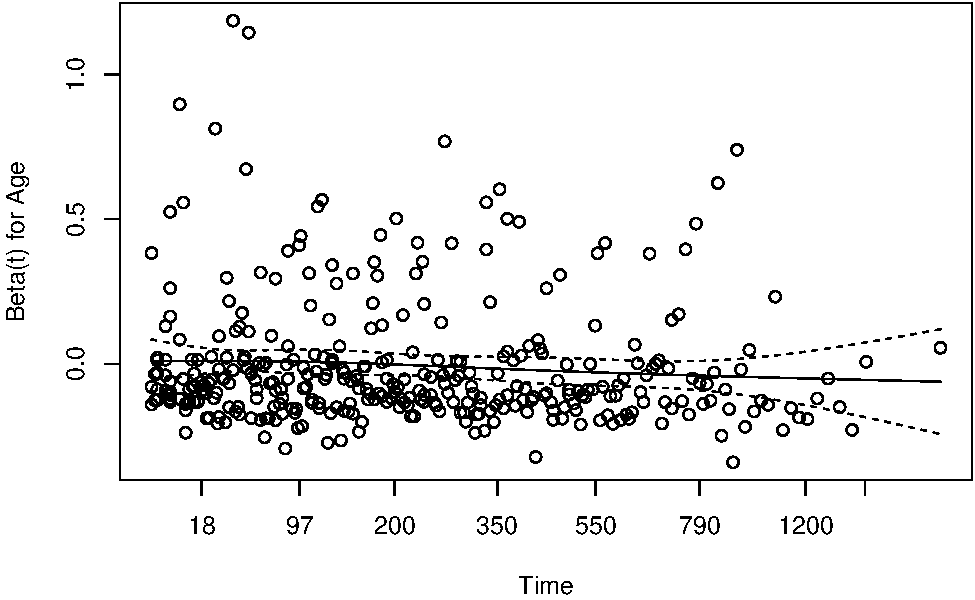
\includegraphics[width=0.32\linewidth]{practical_files/figure-latex/graphical-analysis-1} 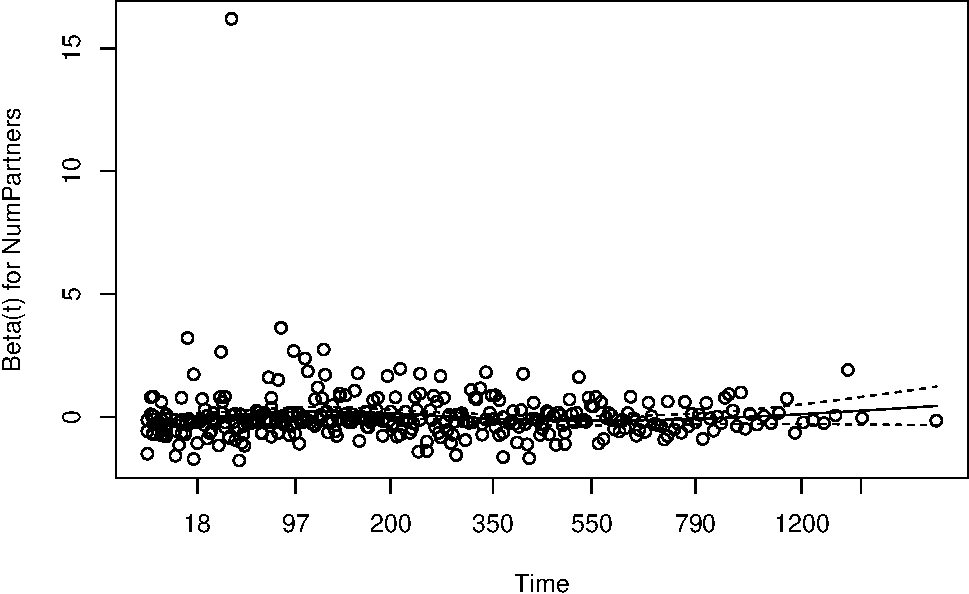
\includegraphics[width=0.32\linewidth]{practical_files/figure-latex/graphical-analysis-2} 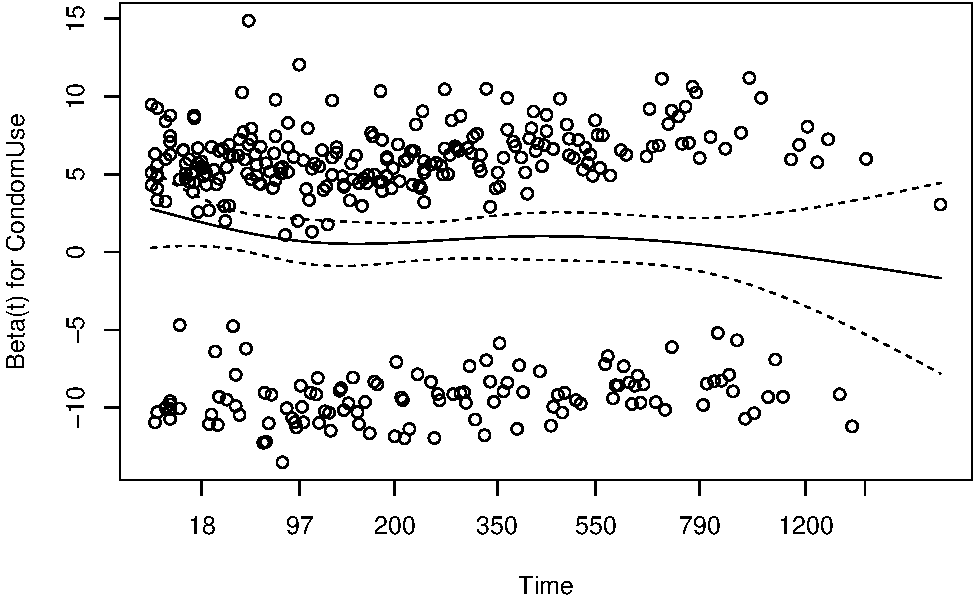
\includegraphics[width=0.32\linewidth]{practical_files/figure-latex/graphical-analysis-3} 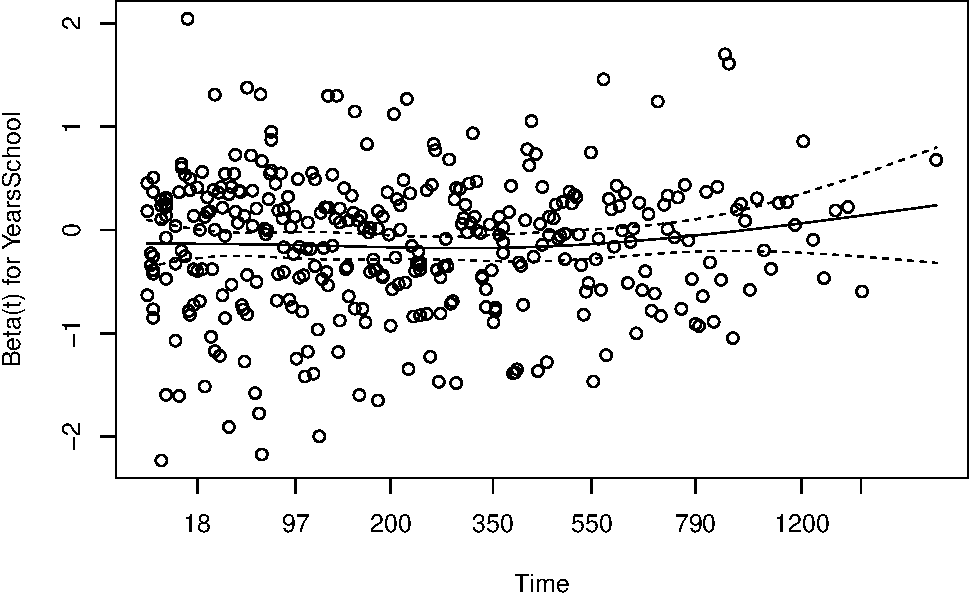
\includegraphics[width=0.32\linewidth]{practical_files/figure-latex/graphical-analysis-4} 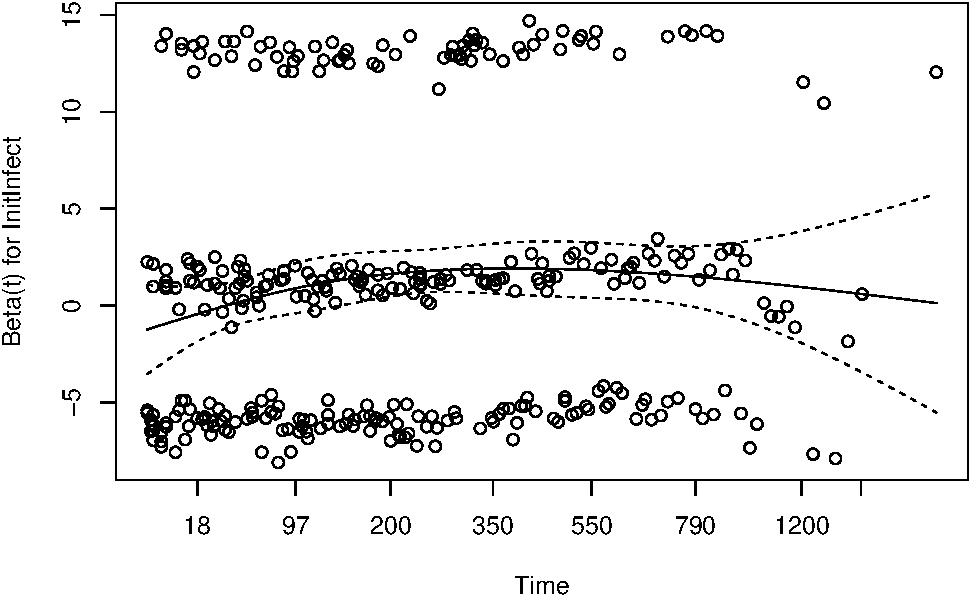
\includegraphics[width=0.32\linewidth]{practical_files/figure-latex/graphical-analysis-5} 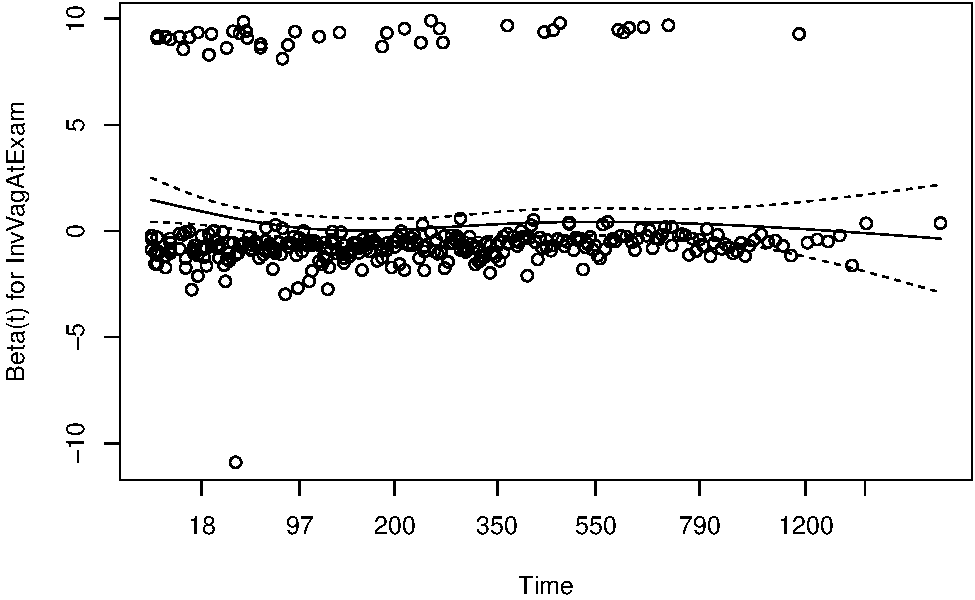
\includegraphics[width=0.32\linewidth]{practical_files/figure-latex/graphical-analysis-6} 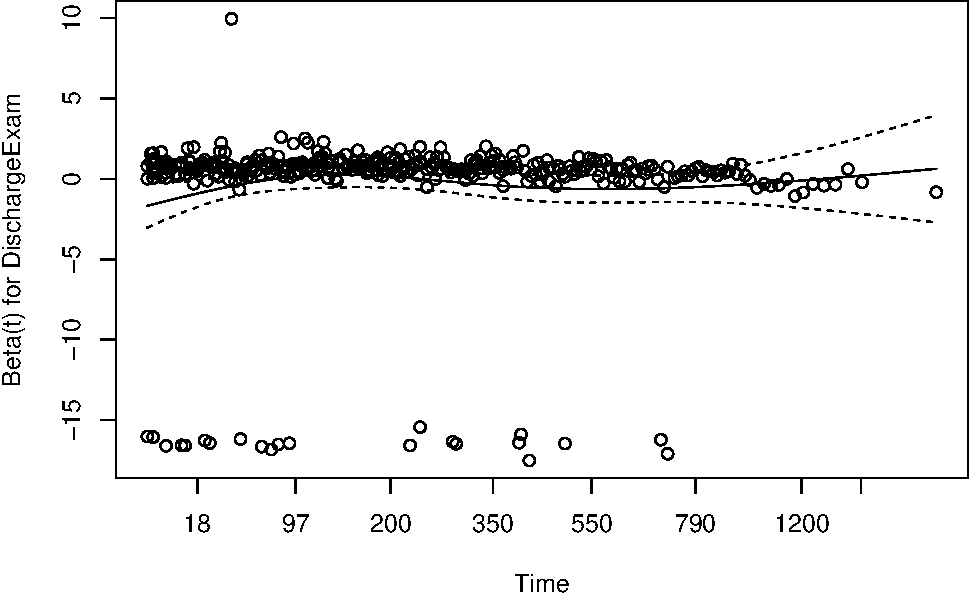
\includegraphics[width=0.32\linewidth]{practical_files/figure-latex/graphical-analysis-7} \caption{Graphical analysis for proportional hazards assumption}\label{fig:graphical-analysis}
\end{figure}

\hypertarget{influential-observations-in-the-global-fit}{%
\subsubsection{Influential Observations in the Global Fit}\label{influential-observations-in-the-global-fit}}

Secondly, we can check if there are any influential observations using residuals based on the score residuals. By plotting a transformation of the score residuals for each of the four coefficients, influential observations can be visually located. More precisely, each plotted residual would be the approximate change in the coefficient vector if the observation in question is dropped, scaled by the standard error of the coefficients. These plots are omitted, but the influential observations that were found are displayed in the output below.

\begin{verbatim}
#>     Age NumPartners CondomUse YearsSchool InitInfect InvVagAtExam DischargeExam
#> 4    43           1         1          12          3            0             1
#> 11   32           6         2          12          3            1             1
#> 154  28           1         2          11          2            0             0
#> 221  18           1         1          11          1            0             1
#> 366  14           1         2           9          1            0             1
#> 498  44           1         3          11          3            0             1
#> 525  15           1         3           8          3            1             1
#> 574  36          19         1          12          3            0             1
#> 831  20          10         2          12          2            1             0
#>     Reinfection TimeUntilReinf
#> 4             1             54
#> 11            0           1468
#> 154           0            880
#> 221           0           1481
#> 366           0           1439
#> 498           1             42
#> 525           0           1005
#> 574           1             43
#> 831           0           1027
\end{verbatim}

By plotting the residuals it was possible to identify as influential observations the individuals with observation numbers: 4, 11, 154, 221, 366, 498, 525, 574 and 831. Individuals 4, 498 and 574 showed a short time until reinfection (in fact below the first quantile of reinfection times), all having close to average amount of schooling, \texttt{InitInfect3} and \texttt{InvVagAtExam0}. The other individuals exhibit a much greater observation time and no reinfection (right censored), with almost all of them having more than 1000 days, even if some of them, e.g.~525 and 11, have \texttt{InvVagAtExam1}.

\hypertarget{linear-covariates-assumption}{%
\subsubsection{Linear Covariates Assumption}\label{linear-covariates-assumption}}

Thirdly, the linear assumption of the continuous variables \texttt{Age}, \texttt{NumPartners} and \texttt{YearsSchool} is checked. This is checked by plotting the residuals from the Cox model when each of the continuous variables are omitted, in addition to a scatter plot smoother. The plots are omitted from the report, but they show that the linear assumption for \texttt{Age} seems to hold fine, while the linear assumption for the other two covariates could be deemed as wrong, since the scatter plot smoother is not flat at all.

\hypertarget{conclusions}{%
\section{Conclusions}\label{conclusions}}

Assuming that the parametric and semi-parametric models can be trusted, the data analysis has uncovered some possible protective factors and risk-factors for reinfection with gonorrhea or chlamydia in women who had suffered one or both infections previously.

\hypertarget{protective-factors}{%
\subsection{Protective Factors}\label{protective-factors}}

The covariates \texttt{YearsSchool} and \texttt{InitInfect2} (Initial infection of Chlamydia only) are statistically significant to a level \(\alpha = 0.05\) in both the parametric and semi-parametric model. Moreover, the logrank tests of the survival curves yield the conclusion that the levels of \texttt{InitInfect} yield different survival curve, which supports the conclusion based on the models. Both these covariates are estimated to being protective factors against reinfection. When it comes to the initial infection of Chlamydia, it is estimated to reduce the instantaneous risk compared to a person with Gonorrhea as initial infection by approximately 32.55\% according to the parametric Weibull model and the Cox-model. Moreover, each unitary increase in \texttt{YearsSchool} is estimated to reduce the instantaneous risk by approximately 12.31\% according to the parametric Weibull model and the Cox-model. Recall that in all these estimations it is assumed that the rest of the profile of each individual is the same, except for the described change.

\hypertarget{risk-factors}{%
\subsection{Risk-factors}\label{risk-factors}}

The covariate \texttt{InvVagAtExam1} (yes) is statistically significant to a level \(\alpha = 0.05\) in both the parametric and semi-parametric model. Moreover, the logrank test of the survival curves yield the conclusion that the levels of the covariate yields different survival curves, which supports the conclusion based on the models. This is estimated to being a risk factor by both models. It is estimated to increasing the instantaneous risk compared a person not experiencing involvement of vagina at exam (with identical profile except for this change) by approximately 48.05\%, when selecting the slightly more optimistic estimate of the Weibull model instead of the more pessimistic estimate from the Cox model 49.47\%.

\end{document}
